\documentclass{../../slides-style}

\slidetitle{Визуальное моделирование, UML}{18.04.2025}

\begin{document}

    \begin{frame}[plain]
        \titlepage
    \end{frame}

    \begin{frame}
        \frametitle{Визуальное моделирование}
        \begin{itemize}
            \item Модели
            \begin{itemize}
                \item Содержат меньше информации, чем код
            \end{itemize}
            \item Метафора моделирования
            \begin{itemize}
                \item Не более чем соглашение между разработчиками
            \end{itemize}
            \item Цель моделирования
            \begin{itemize}
                \item Каждая модель существует для кого-то и для чего-то
                \item Модели как средства общения, как документация и как графические исходники
            \end{itemize}
        \end{itemize}
    \end{frame}

    \begin{frame}
        \frametitle{Пример модели}
        \begin{center}
            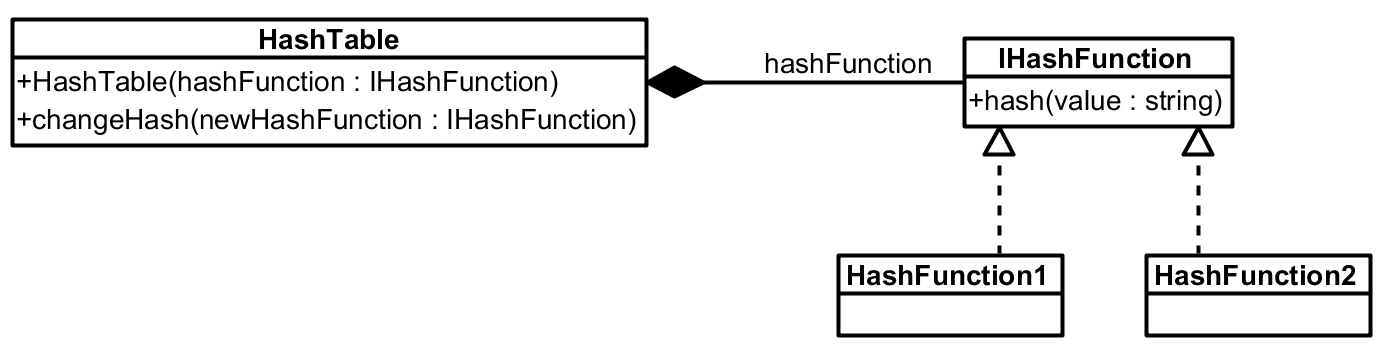
\includegraphics[width=0.9\textwidth]{modelExample.png}
        \end{center}
    \end{frame}

    \begin{frame}
        \frametitle{Unified Modeling Language}
        \begin{itemize}
            \item Семейство графических нотаций
            \begin{itemize}
                \item 14 видов диаграмм
            \end{itemize}
            \item Общая метамодель
            \item Стандарт под управлением Object Management Group
            \begin{itemize}
                \item UML 1.1 --- 1997 год
                \item UML 2.5.1 --- декабрь 2017 года
            \end{itemize}
            \item Прежде всего, для проектирования ПО
        \end{itemize}
    \end{frame}

    \begin{frame}
        \frametitle{Книжка}
        \begin{columns}
            \begin{column}{0.5\textwidth}
                \begin{center}
                    
\includegraphics[width=0.4\textwidth]{umlBookCover.png}
                \end{center}
            \end{column}
            \begin{column}{0.5\textwidth}
                М. Фаулер, UML. Основы. Краткое руководство по стандартному языку объектного моделирования. СПб., Символ-Плюс, 2011. 192 С.
            \end{column}
        \end{columns}
    \end{frame}

    \begin{frame}
        \frametitle{Диаграммы UML}
        \begin{center}
            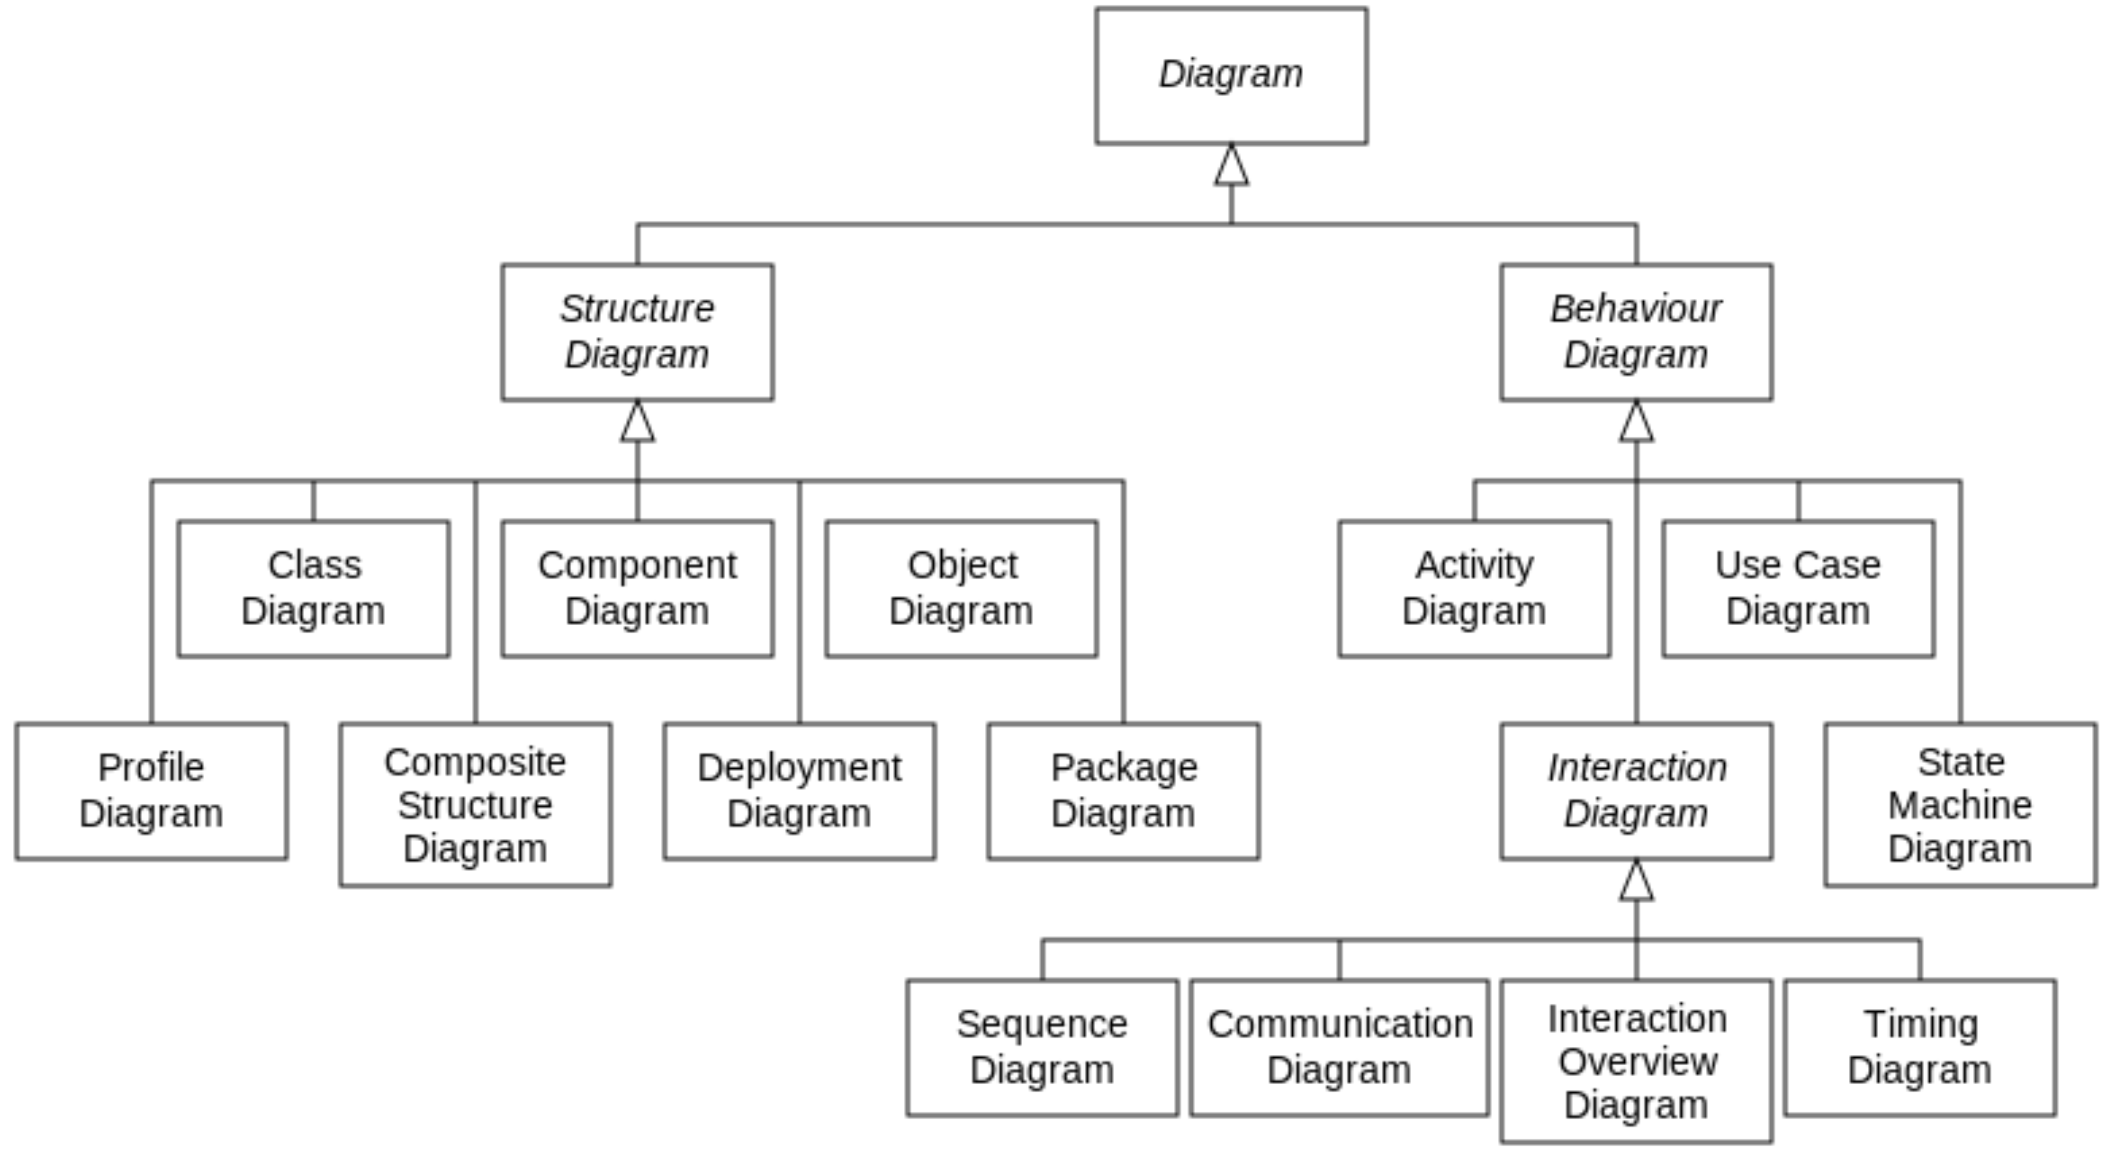
\includegraphics[width=0.9\textwidth]{umlDiagrams.png}
        \end{center}
    \end{frame}

    \begin{frame}
        \frametitle{Диаграммы классов UML}
        \begin{center}
            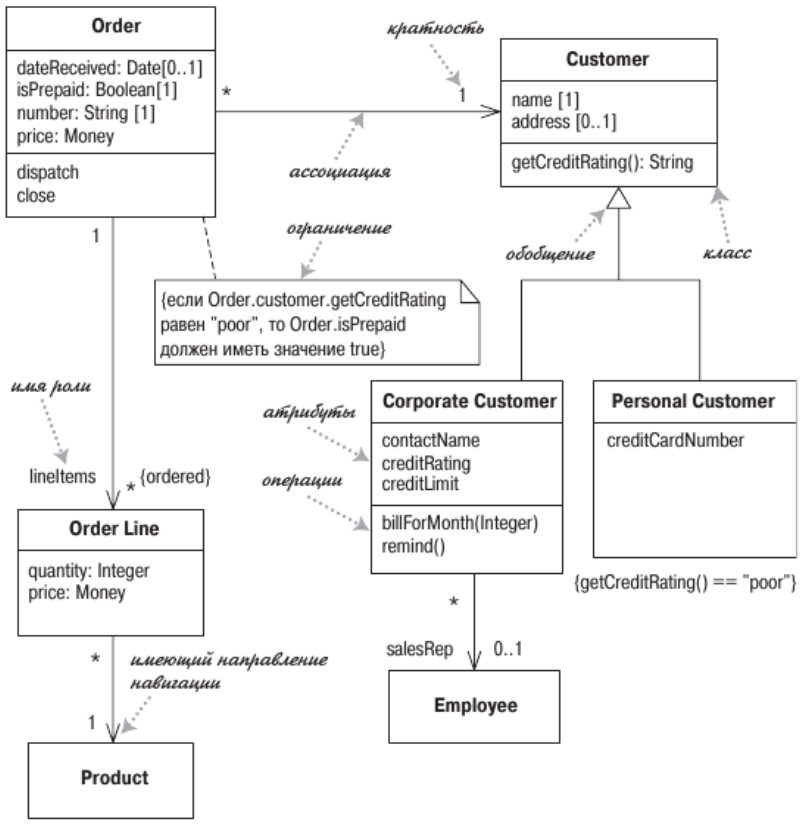
\includegraphics[width=0.6\textwidth]{umlClassDiagram.png}
            \attribution{М. Фаулер. ``UML. Основы''}
        \end{center}
    \end{frame}

    \begin{frame}[fragile]
        \frametitle{Как это связано с кодом}
        \begin{columns}
            \begin{column}{0.5\textwidth}
                \begin{footnotesize}
                    \begin{minted}{java}
public class OrderLine {
    private int quantity;
    private Product product;
    public int getQuantity() {
        return quantity;
    }
    public void setQuantity(int quantity) {
        this.quantity = quantity;
    }
    public Money getPrice() {
        return product.getPrice().multiply(quantity);
    }
}
                    \end{minted}
                \end{footnotesize}
            \end{column}
            \begin{column}{0.5\textwidth}
                \begin{center}
                    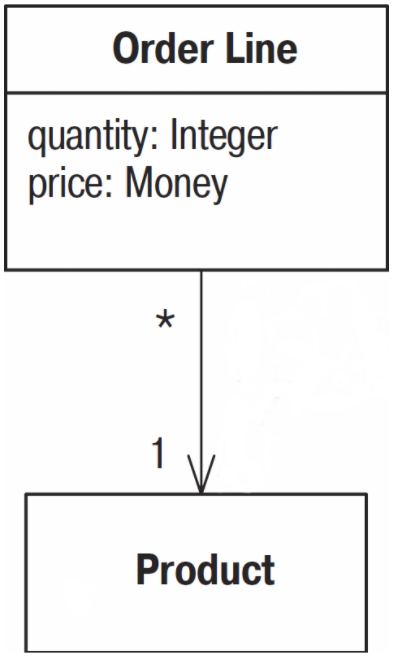
\includegraphics[width=0.5\textwidth]{orderLine.png}
                \end{center}
            \end{column}
        \end{columns}
    \end{frame}

    \begin{frame}
        \frametitle{Свойства}
        \begin{columns}
            \begin{column}{0.3\textwidth}
                \begin{center}
                    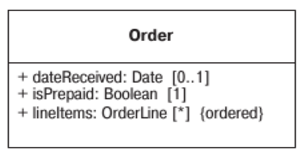
\includegraphics[width=0.8\textwidth]{attributes.png}

                    Атрибуты
                \end{center}
            \end{column}
            \begin{column}{0.7\textwidth}
                \begin{center}
                    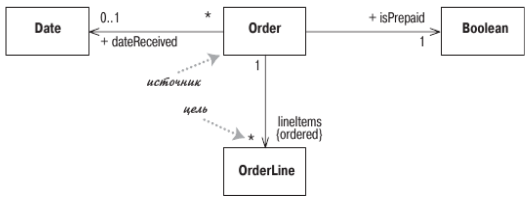
\includegraphics[width=0.7\textwidth]{associations.png}

                    Ассоциации
                \end{center}
            \end{column}
        \end{columns}
        \bigskip
        Синтаксис:
        \begin{itemize}
            \item видимость имя: тип кратность = значение по умолчанию \{строка свойств\}
            \item Видимость: + (public), - (private), \# (protected), \char`~ (package)
            \item Кратность: 1 (ровно 1 объект), 0..1 (ни одного или один),\newline * (сколько угодно), 1..*, 2..*
        \end{itemize}
    \end{frame}

    \begin{frame}
        \frametitle{Агрегация и композиция}
        Агрегация – объект ``знает'' о другом (не управляет его временем жизни, имеет на него ссылку)
        \begin{center}
            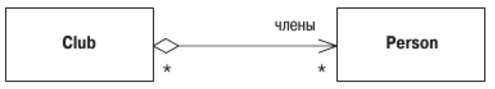
\includegraphics[width=0.5\textwidth]{aggregations.png}
        \end{center}
        Композиция --- объект владеет другим объектом (управляет его временем жизни, хранит его по значению или по указателю, делая delete)
        \begin{center}
            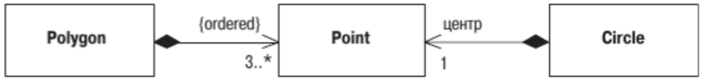
\includegraphics[width=0.7\textwidth]{compositions.png}
        \end{center}
        Уточнение обычной ассоциации, используется только если очень надо
    \end{frame}

    \begin{frame}
        \frametitle{Агрегация и композиция, пример}
        \begin{center}
            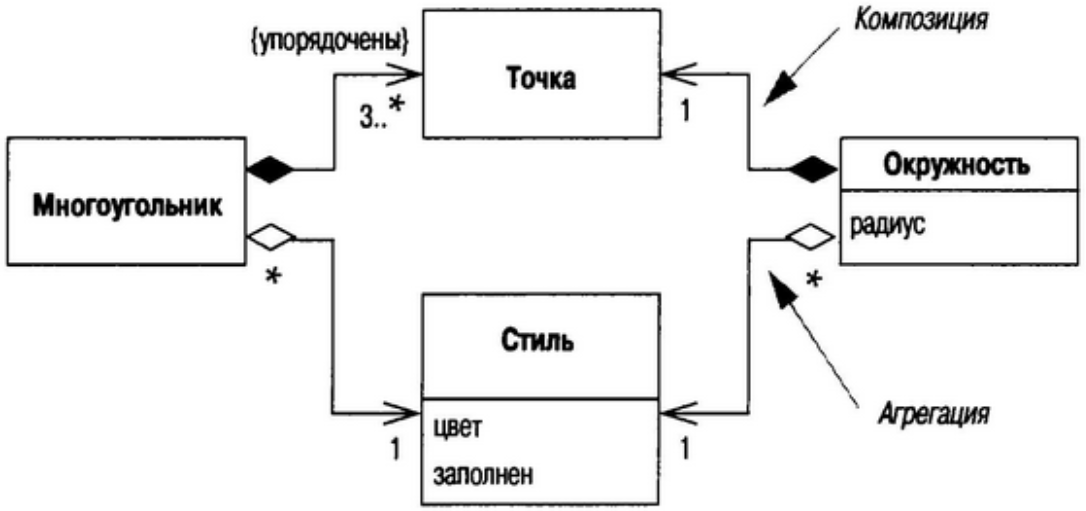
\includegraphics[width=0.7\textwidth]{aggregationAndCompositionExample.png}
            \attribution{М. Фаулер. ``UML. Основы''}
        \end{center}
    \end{frame}

    \begin{frame}
        \frametitle{Прочее}
        \begin{columns}
            \begin{column}{0.5\textwidth}
                \begin{center}
                    Интерфейсы

                    \bigskip
                    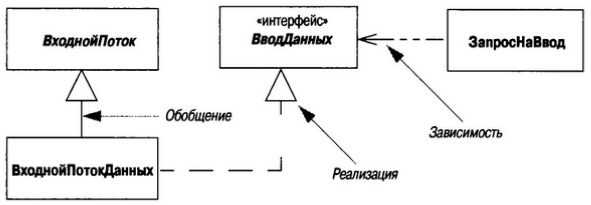
\includegraphics[width=0.9\textwidth]{interfaces1.png}

                    \bigskip
                    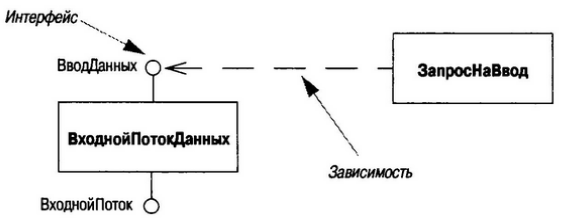
\includegraphics[width=0.9\textwidth]{interfaces2.png}
                \end{center}
            \end{column}
            \begin{column}{0.5\textwidth}
                \begin{center}
                    Зависимости

                    \bigskip
                    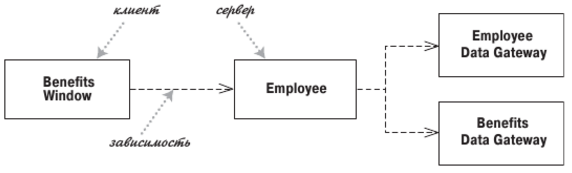
\includegraphics[width=0.9\textwidth]{dependencies.png}
                    \bigskip

                    Шаблоны

                    \bigskip
                    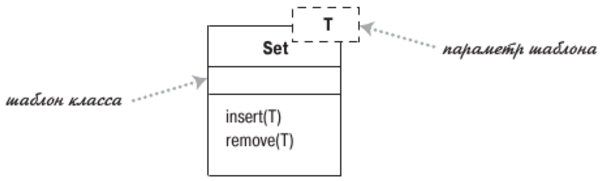
\includegraphics[width=0.9\textwidth]{templates.png}
                \end{center}
            \end{column}
        \end{columns}
    \end{frame}

    \begin{frame}
        \frametitle{Диаграммы компонентов}
        \framesubtitle{Component diagrams}
        \begin{center}
            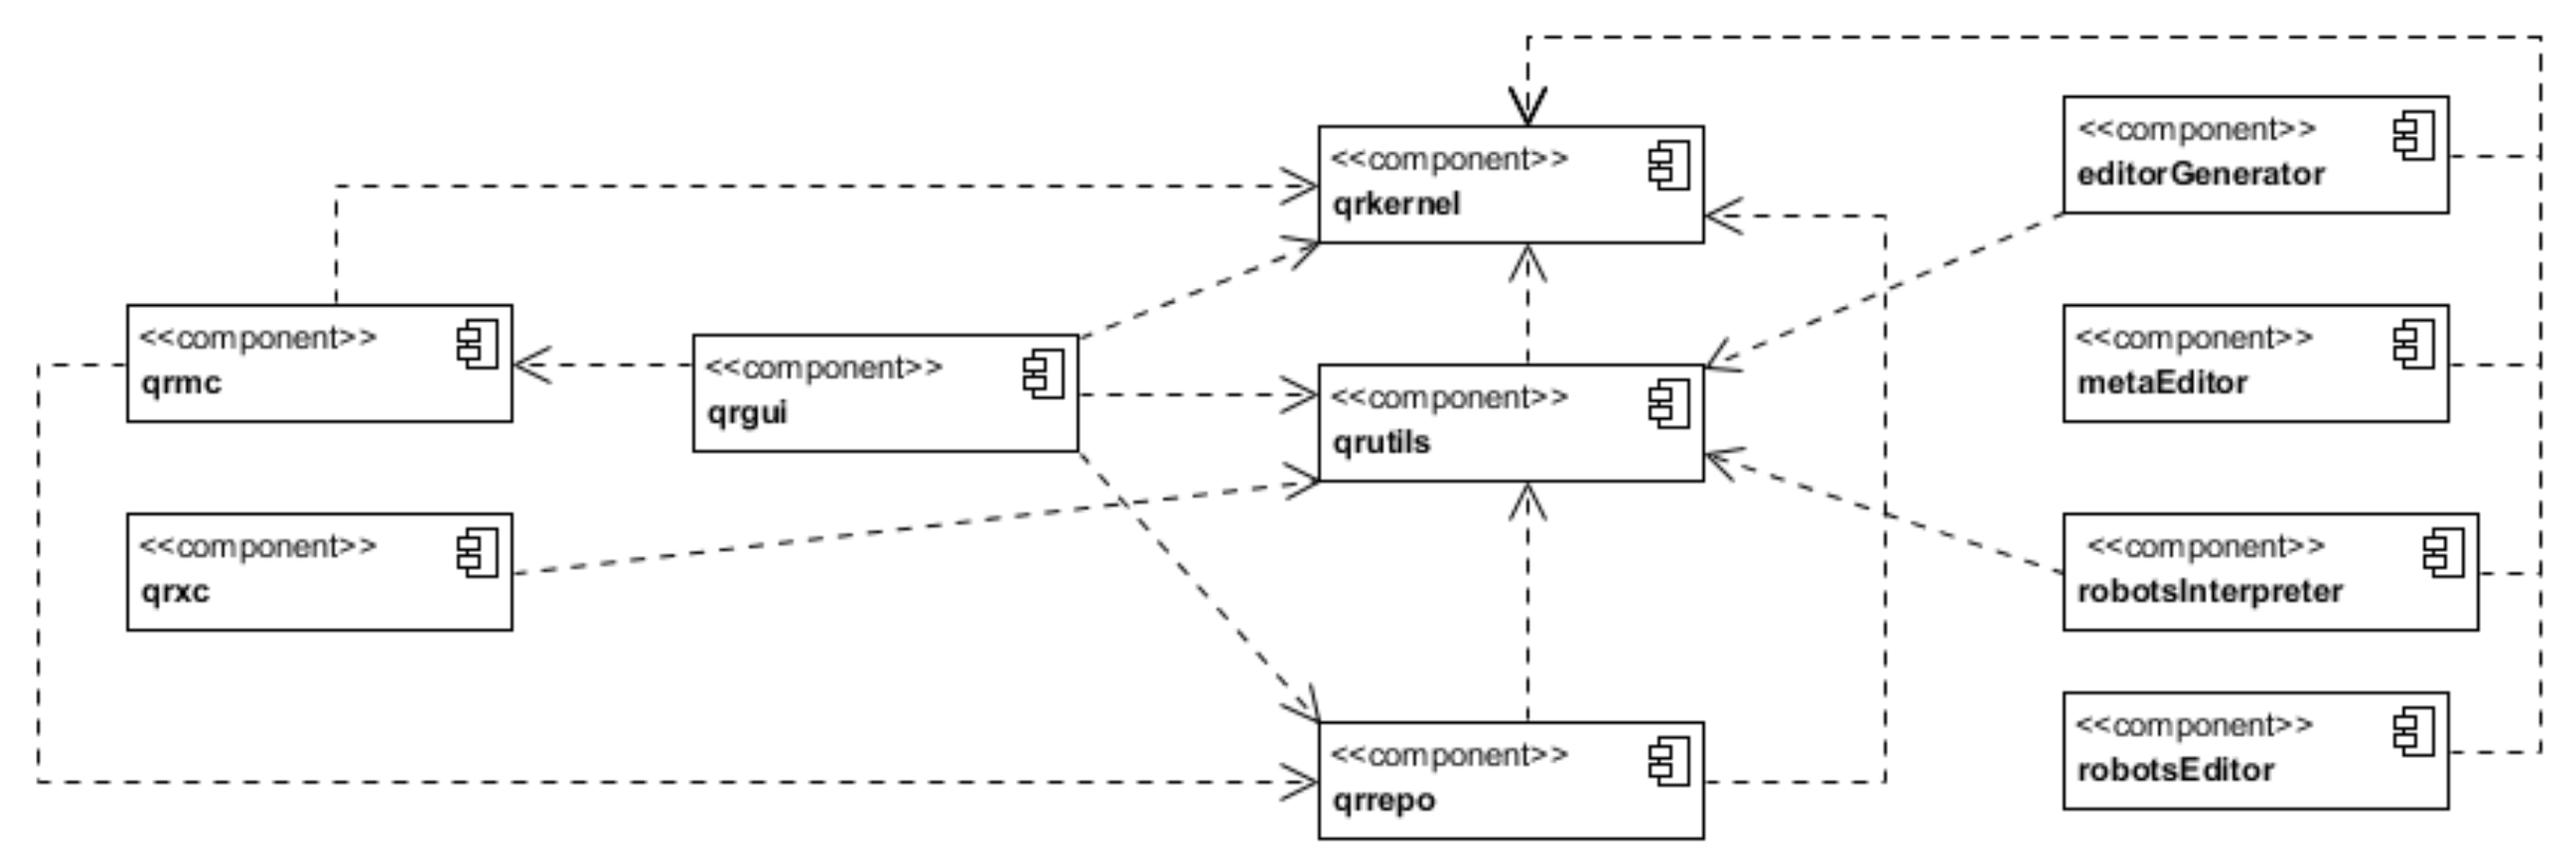
\includegraphics[width=0.9\textwidth]{componentDiagram.png}
        \end{center}
    \end{frame}

    \begin{frame}
        \frametitle{Более подробно}
        \begin{center}
            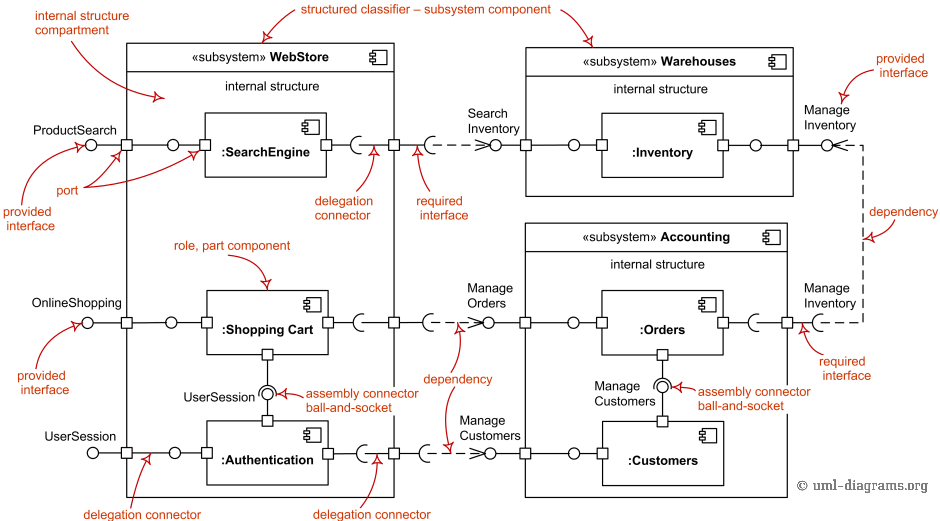
\includegraphics[width=0.95\textwidth]{componentDiagramsOverview.png}
            \attribution{\url{http://www.uml-diagrams.org}}
        \end{center}
    \end{frame}

    \begin{frame}
        \frametitle{Диаграммы случаев использования}
        \framesubtitle{Use case diagrams}
        \begin{center}
            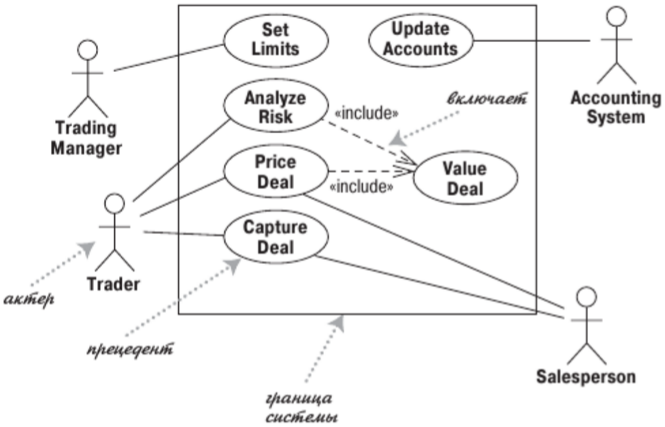
\includegraphics[width=0.6\textwidth]{useCaseDiagram.png}
        \end{center}
    \end{frame}

    \begin{frame}
        \frametitle{Диаграммы активностей}
        \framesubtitle{Activity diagrams}
        \begin{center}
            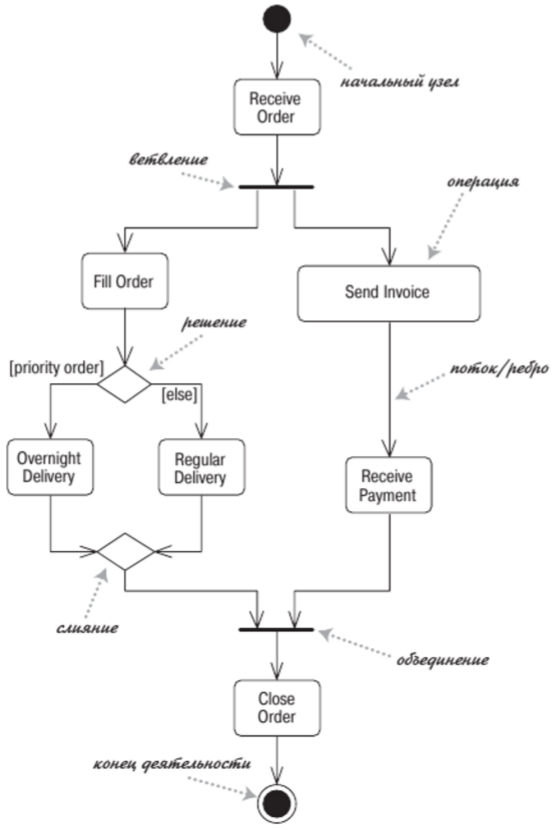
\includegraphics[width=0.415\textwidth]{activityDiagram.png}
        \end{center}
    \end{frame}

    \begin{frame}
        \frametitle{Диаграммы последовательностей}
        \framesubtitle{Sequence diagrams}
        \begin{center}
            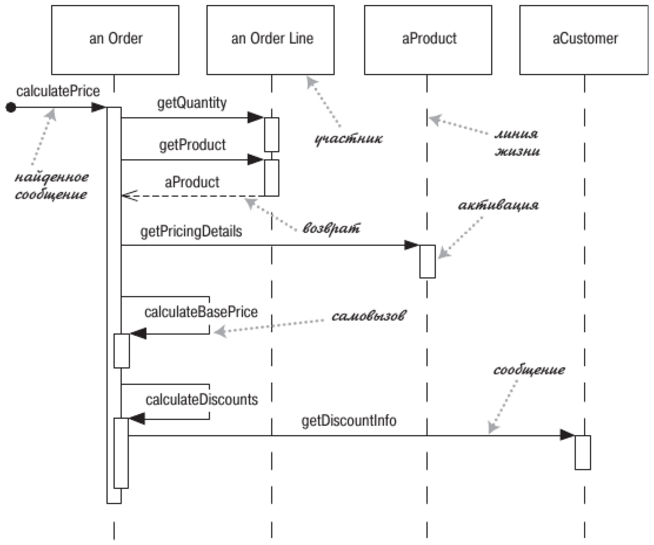
\includegraphics[width=0.6\textwidth]{sequenceDiagram.png}
        \end{center}
    \end{frame}

    \begin{frame}
        \frametitle{Диаграммы конечных автоматов}
        \framesubtitle{State diagrams}
        \begin{columns}
            \begin{column}{0.5\textwidth}
                \begin{itemize}
                    \item Состояние
                    \begin{itemize}
                        \item entry activity
                        \item exit activity
                        \item do activity
                        \item внутренний переход
                    \end{itemize}
                    \item Событие
                    \item Переход
                    \begin{itemize}
                        \item имя события (список параметров) [сторожевое условие] выражение действия
                    \end{itemize}
                \end{itemize}
            \end{column}
            \begin{column}{0.5\textwidth}
                \begin{center}
                    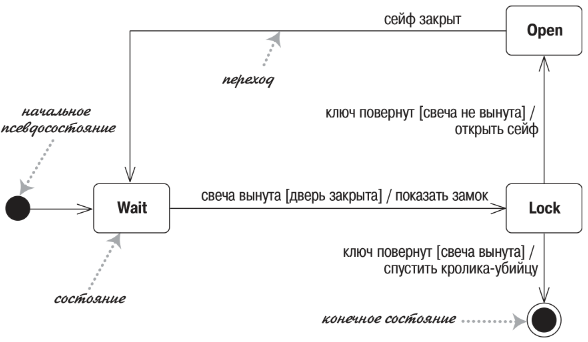
\includegraphics[width=\textwidth]{stateTransitionSyntax.png}
                    \attribution{М. Фаулер, UML. Основы}
                \end{center}
            \end{column}
        \end{columns}
    \end{frame}

    \begin{frame}[fragile]
        \frametitle{Генерация кода}
        \begin{columns}
            \begin{column}{0.5\textwidth}
                \begin{tiny}
                    \begin{minted}{java}
public void handleEvent(PanelEvent anEvent) {
    switch (currentState) {
        case PanelState.Open:
            switch (anEvent) {
                case PanelEvent.SafeClosed:
                    currentState = PanelState.Wait;
            }
            break;
        case PanelState.Wait:
            switch (anEvent) {
                case PanelEvent.CandleRemoved:
                    if (isDoorOpen) {
                        revealLock();
                        currentState = PanelState.Lock;
                    }
            }
            break;
        case PanelState.Lock:
            switch (anEvent) {
                case PanelEvent.KeyTurned:
                    if (isCandleIn) {
                        openSafe();
                        currentState = PanelState.Open;
                    } else {
                        releaseKillerRabbit();
                        currentState = PanelState.Final;
                    }
            }
            break;
    }
}
                    \end{minted}
                \end{tiny}
            \end{column}
            \begin{column}{0.5\textwidth}
                \begin{center}
                    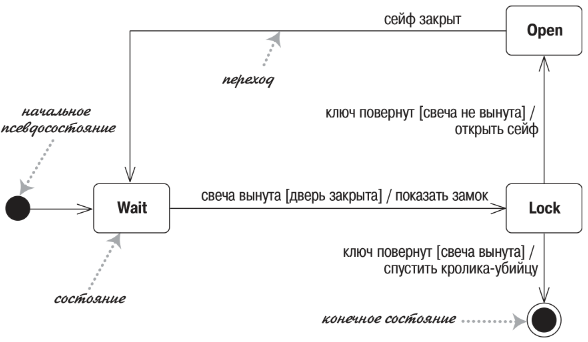
\includegraphics[width=\textwidth]{stateTransitionSyntax.png}
                    \attribution{М. Фаулер, UML. Основы}
                \end{center}
            \end{column}
        \end{columns}
    \end{frame}

    \begin{frame}
        \frametitle{Таблица состояний}
        \begin{center}
            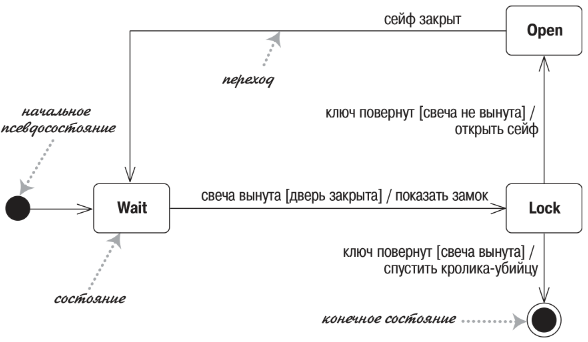
\includegraphics[width=0.4\textwidth]{stateTransitionSyntax.png}
        \end{center}

        \begin{center}
            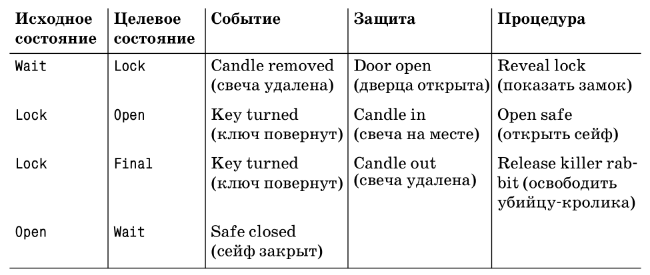
\includegraphics[width=0.5\textwidth]{stateTransitionStateTable.png}
            \attribution{М. Фаулер, UML. Основы}
        \end{center}
    \end{frame}

    \begin{frame}
        \frametitle{Паттерн ``Состояние''}
        \begin{center}
            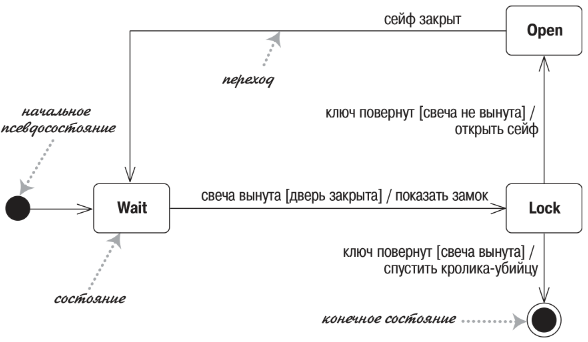
\includegraphics[width=0.4\textwidth]{stateTransitionSyntax.png}
        \end{center}

        \begin{center}
            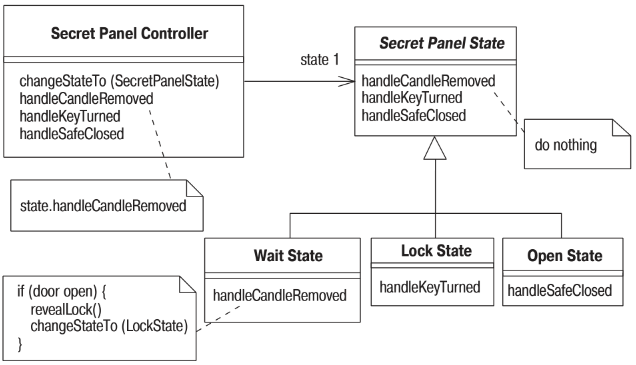
\includegraphics[width=0.5\textwidth]{stateTransitionStatePattern.png}
            \attribution{М. Фаулер, UML. Основы}
        \end{center}
    \end{frame}

    \begin{frame}
        \frametitle{Диаграммы развёртывания}
        \framesubtitle{Deployment diagrams}
        \begin{columns}
            \begin{column}{0.5\textwidth}
                \begin{itemize}
                    \item Показывает отображение компонентов и физических артефактов на реальные (или виртуальные) устройства
                    \item Бывает полезна на начальных этапах проектирования, даже до диаграмм компонентов
                \end{itemize}
            \end{column}
            \begin{column}{0.5\textwidth}
                \begin{center}
                    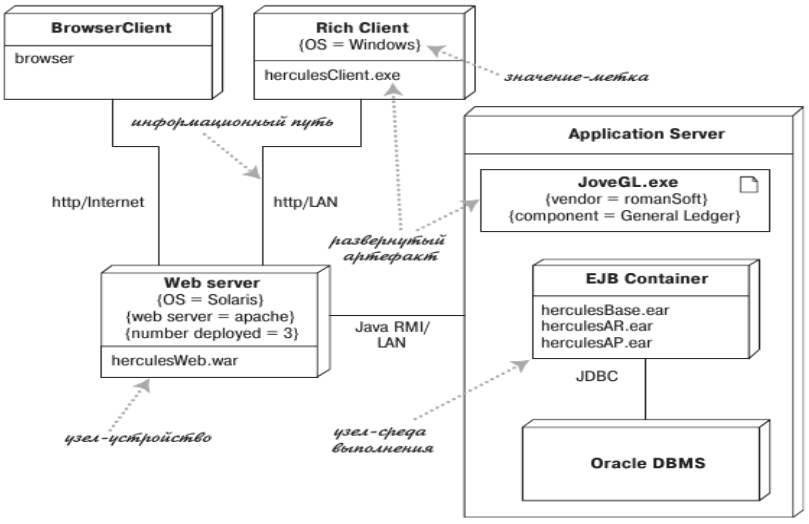
\includegraphics[width=\textwidth]{deploymentDiagram.png}
                    \attribution{М. Фаулер, UML. Основы}
                \end{center}
            \end{column}
        \end{columns}
    \end{frame}

    \begin{frame}
        \frametitle{Примеры CASE-инструментов}
        \begin{itemize}
            \item ``Рисовалки''
            \begin{itemize}
                \item Visio
                \item Dia
                \item SmartDraw
                \item LucidChart
                \item Creately
                \item \url{http://diagrams.net/}
            \end{itemize}
            \item Полноценные CASE-системы
            \begin{itemize}
                \item Enterprise Architect
                \item Rational Software Architect
                \item MagicDraw
                \item Visual Paradigm
                \item GenMyModel
            \end{itemize}
            \item Текстовые редакторы
            \begin{itemize}
                \item \url{https://www.websequencediagrams.com/}
                \item \url{http://yuml.me/}
                \item \url{http://plantuml.com/}
            \end{itemize}
        \end{itemize}
    \end{frame}

    \begin{frame}
        \frametitle{Предметно-ориентированные языки}
        \begin{center}
            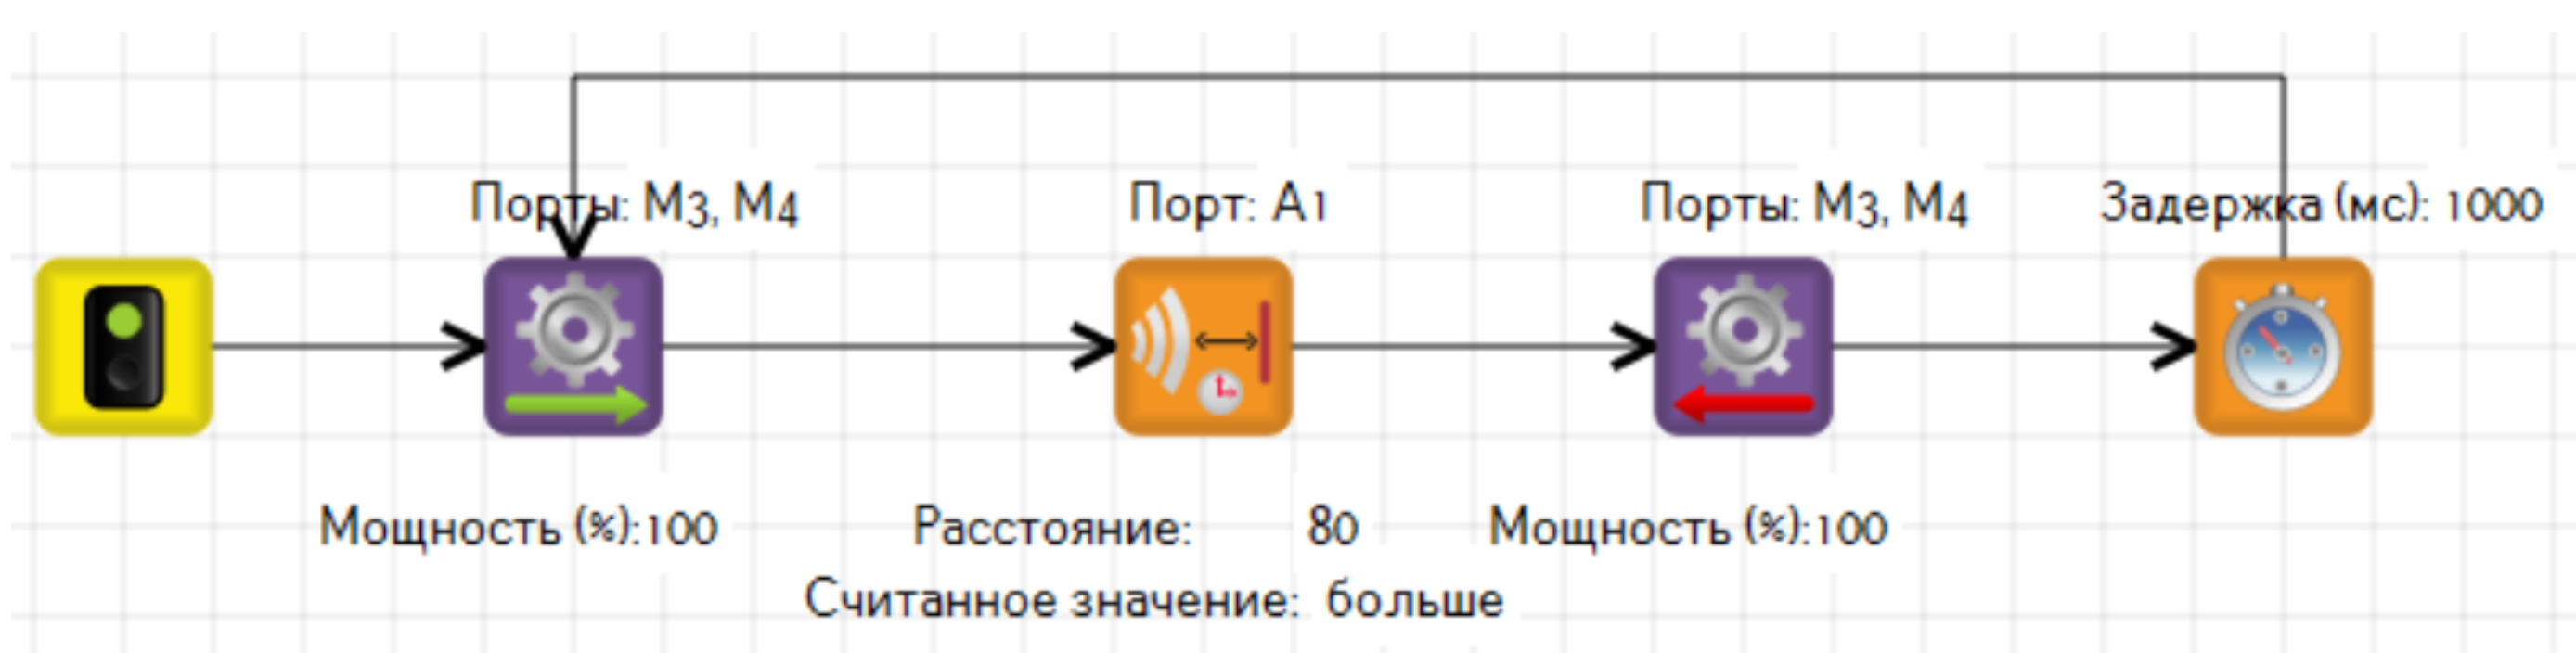
\includegraphics[width=0.9\textwidth]{domainLanguages.png}
        \end{center}
    \end{frame}

\end{document}
